\documentclass[12pt, a4paper]{article}

% --- PACCHETTI ---
\usepackage[utf8]{inputenc}
\usepackage[italian]{babel}
\usepackage{graphicx}
\usepackage{listings}
\usepackage{xcolor}
\usepackage{hyperref}
\usepackage{geometry}

% --- CONFIGURAZIONE PAGINA ---
\geometry{margin=2.5cm}

% --- CONFIGURAZIONE CODICE JAVA ---
\definecolor{codegreen}{rgb}{0,0.6,0}
\definecolor{codegray}{rgb}{0.5,0.5,0.5}
\definecolor{codepurple}{rgb}{0.58,0,0.82}
\definecolor{backcolour}{rgb}{0.97,0.97,0.95}

\lstset{
    backgroundcolor=\color{backcolour},
    commentstyle=\color{codegreen},
    keywordstyle=\color{blue},
    numberstyle=\tiny\color{codegray},
    stringstyle=\color{codepurple},
    basicstyle=\ttfamily\footnotesize,
    breakatwhitespace=false,
    breaklines=true,
    captionpos=b,
    keepspaces=true,
    numbers=left,
    numbersep=5pt,
    showspaces=false,
    showstringspaces=false,
    showtabs=false,
    tabsize=2,
    language=Java
}

\title{Relazione Progetto: Sistema Gestione Biblioteca \\ \large Ingegneria del Software}
\author{Studente: Marco}
\date{15 Maggio 2026}

\begin{document}

\maketitle

\begin{abstract}
La presente relazione documenta lo sviluppo di un sistema software per la gestione di una biblioteca, focalizzandosi sull'applicazione pratica dei principi di ingegneria del software: analisi dei requisiti, modellazione UML, implementazione in Java 21 e verifica tramite testing automatizzato.
\end{abstract}

\tableofcontents
\newpage

\section{Introduzione}
Il sistema ha l'obiettivo di informatizzare i processi principali di una biblioteca universitaria, nello specifico la consultazione del catalogo e la gestione del prestito dei volumi.

\section{Analisi dei Requisiti}
\subsection{Requisiti Funzionali (Casi d'Uso)}
Il sistema risponde ai seguenti casi d'uso principali:
\begin{itemize}
    \item \textbf{UC1 - Ricerca Libro:} Permette di interrogare il catalogo per verificare la presenza di un titolo.
    \item \textbf{UC2 - Richiesta Prestito:} Gestisce l'assegnazione temporanea di un libro a un utente.
\end{itemize}

\subsection{Requisiti Non Funzionali e Criteri di Accettazione}
Come richiesto dai vincoli comuni del progetto:
\begin{itemize}
    \item \textbf{Affidabilità:} Il sistema garantisce l'integrità impedendo prestiti duplicati dello stesso volume.
    \item \textbf{Manutenibilità:} Struttura modulare con responsabilità chiare per facilitare evoluzioni future.
    \item \textbf{Criterio di Accettazione (Prestito):} Il prestito deve fallire (restituendo \textit{false}) se il libro è già impegnato.
    \item \textbf{Criterio di Accettazione (Ricerca):} La ricerca deve avere successo anche con titoli parziali (case-insensitive).
\end{itemize}

\begin{figure}[ht]
    \centering
    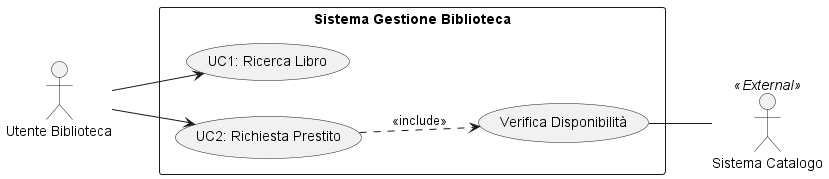
\includegraphics[width=0.75\textwidth]{images/casi_uso.png}
    \caption{Diagramma dei Casi d'Uso del Sistema.}
\end{figure}

\section{Design del Sistema}
\subsection{Architettura e Principi SOLID}
L'architettura applica in modo ragionato i principi SOLID:
\begin{itemize}
    \item \textbf{Single Responsibility Principle (SRP):} La classe \texttt{GestorePrestiti} si occupa solo della logica di transazione, separata dal modello dei dati (\texttt{Libro}/\texttt{Utente}).
    \item \textbf{Open-Closed Principle (OCP):} Il design permette di aggiungere nuove funzionalità al catalogo senza modificare il core del gestore prestiti.
    \item \textbf{Dependency Inversion Principle (DIP):} Le dipendenze tra moduli sono ridotte per favorire il testing unitario.
\end{itemize}

\begin{figure}[ht]
    \centering
    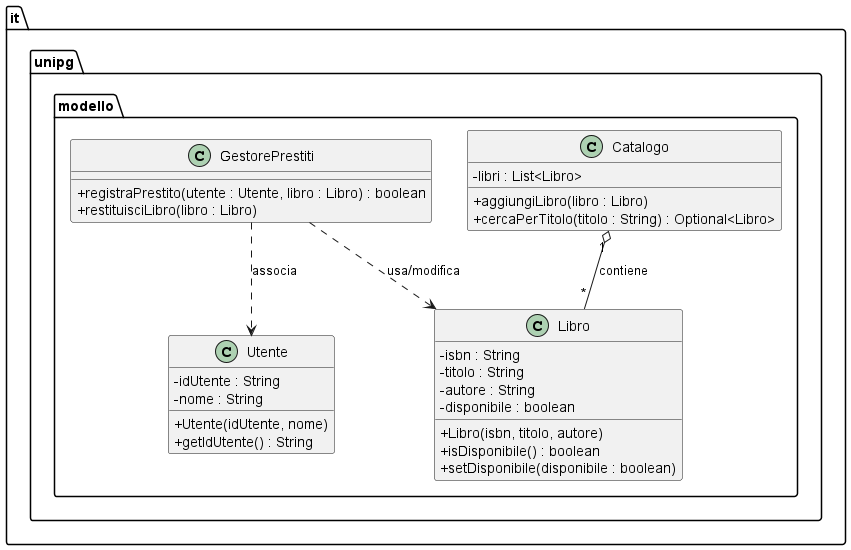
\includegraphics[width=0.85\textwidth]{images/classi.png}
    \caption{Diagramma delle Classi - Struttura e Relazioni.}
\end{figure}

\subsection{Matrice di Tracciabilità}
Per garantire il collegamento tra requisiti, codice e test:
\begin{table}[h]
\centering
\begin{tabular}{|l|l|l|}
\hline
\textbf{Caso d'Uso} & \textbf{Implementazione} & \textbf{Test Unitario} \\ \hline
UC1: Ricerca Libro & Catalogo.java & CatalogoTest.java \\ \hline
UC2: Richiesta Prestito & GestorePrestiti.java & GestorePrestitiTest.java \\ \hline
\end{tabular}
\caption{Matrice di Tracciabilità.}
\end{table}

\section{Implementazione Tecnologica}
\subsection{Ambiente di Sviluppo}
\begin{itemize}
    \item \textbf{JDK}: Java 21 (LTS).
    \item \textbf{Build Tool}: Maven 3.x.
    \item \textbf{Testing}: JUnit 5 (Jupiter).
\end{itemize}

\subsection{Snippet di Codice Significativo}
\begin{lstlisting}[caption={Logica di validazione del prestito in GestorePrestiti.java }]
public boolean registraPrestito(Utente utente, Libro libro) {
    if (libro.isDisponibile()) {
        libro.setDisponibile(false);
        return true;
    }
    return false;
}
\end{lstlisting}

\section{Verifica e Validazione}
\subsection{Risultati dei Test}
L'esecuzione del comando \texttt{mvn clean test} conferma il superamento dei test per flussi positivi e di errore:
\begin{itemize}
    \item \textbf{Test eseguiti}: 4 su 4 superati (100\%).
    \item \textbf{Stato finale}: BUILD SUCCESS.
\end{itemize}

\section{Conclusioni}
Il progetto soddisfa i requisiti minimi di implementazione end-to-end, qualità del design (SOLID) e documentazione richiesti.

\end{document}